\section{Návrh schématu}

Tato kapitola se zabývá návrhem schématu tištěného spoje. Zapojení je rozděleno do čtyř logických prvků. Jedná se o první verzi schématu.
\subsection{Tvorba vlastních symbolů}
\begin{wrapfigure}{l}{0.3\textwidth}% příklad symbolu
    
\includegraphics[width = 0.3\textwidth]{H-bridge.png}
    \label{custom_kicad_symbol}
    \caption{Vlastní symbol KiCAD, H můstek}
\end{wrapfigure}
KiCAD neobsahuje symboly všech součástek na světě. Není to totiž reálné. Občas je tedy nutné vytvořit si vlastní symboly pro své součástky. Pro tuto práci bylo vytvořeno několik symbolů. Symbol pro step up moduly, symbol pro ochranu baterií a symbol pro akcelerometr.
\newline
\subsection{Celek}
Tato podkapitola popisuje vztahy mezi podschématy pomocí hirearchických štítků.
Propojuje usb převodník s ESP32 pomocí UART sériové komunikace. Dále propojuje výstup Power Delivery input schématu s nabíječkou 18650 článků nacházející se ve schématu PSU. Z PSU napájí H můstky, které jsou uvnitř propojeny s motory.  H můstky jsou dále propojeny s řídící částí H můstků a se zpětnou vazbou motorů. ESP32 ještě monitoruje napětí 18650 článků a vyhodnocuje hladinu nabití baterií. ze schématu logika obsahujícího ESP je také vyvedena příprava pro neopixel diody a sériová komunikace pro rozšiřující moduly.

\newpage
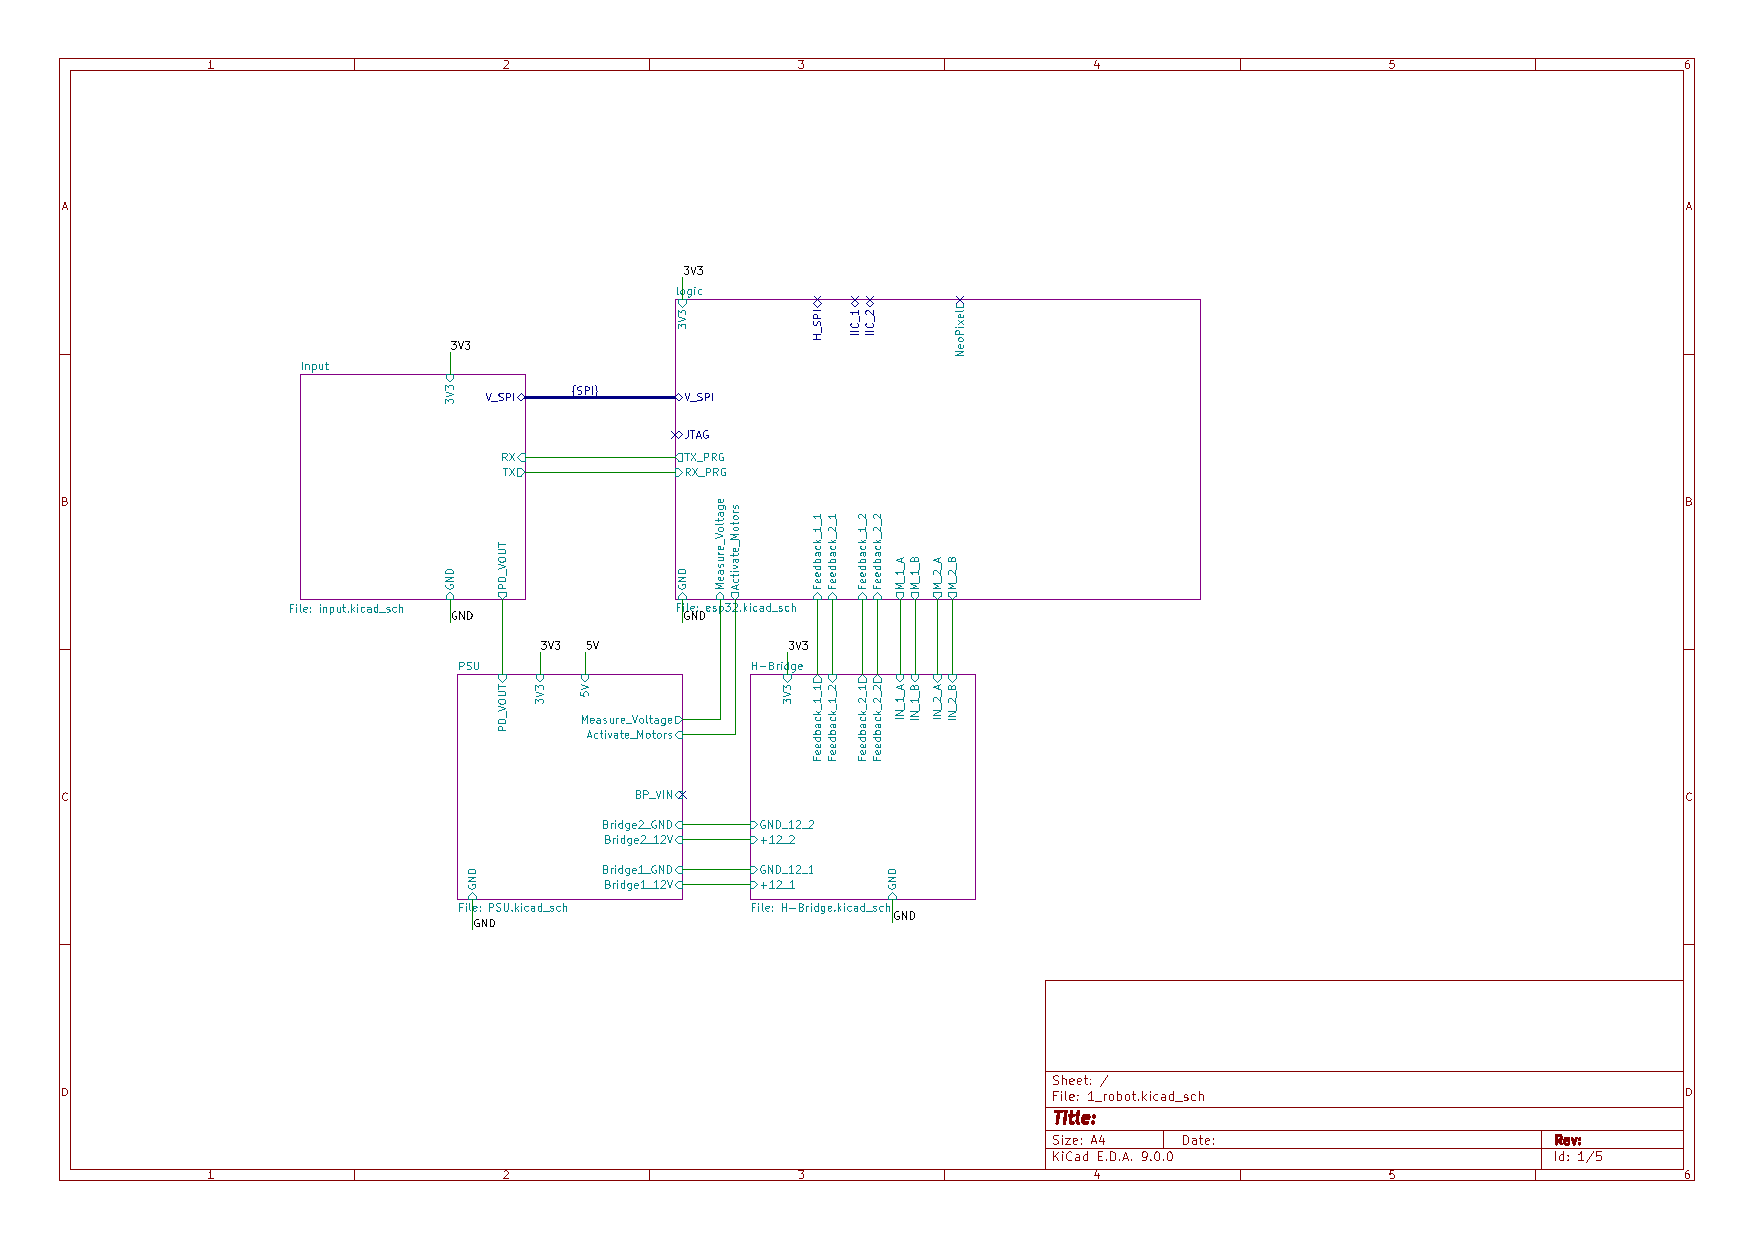
\includepdf[angle = -90]{obrazky/old_schematic.pdf}

\subsection{Vstupy}
Schéma vstupy převádí signál USB na UART, přes který následně probíhá komunikace s ESP32 modulem. 
Nachází se zde také schéma pro Power Delivery, přes které je následně možnost napájení celého robota. Power delivery je protokol pro aktivní řízení napájecího napětí. Zařízení přípojené ke kompatibilnímu zdroji dokáže vykomunikovat napětí v rozmetí 5-20V. V ojedinělých případech tento protokol podporuje napětí až 48V. Při proudu 5A se poté jedná o příkon až 240W. Integrovaný obvod AP33771DKZ však podporuje maximálně 100w nabíjení pomocí 20W. Tento robot vžak využívá 8.6V a maximální nabíjecí proud je omezen na 18W.


\newpage
\includepdf[angle = -90]{obrazky/old_schematic-input.pdf}

\subsection{H-můstky}

H můstky jsou používány pro řízení směru a rychlosti otáčení motorů pomocí PWM signálu, jenž generuje Mikrokontroler ESP32.
Dále se zde nachází konektory pro připojení motorů. Je využita kombinace 4pinového a 2 pinového konektoru. Pro připojení je potřeba pinů šest. Proč tedy nebyl použit šestipinový konektor? Takto velký konektor se bohužel nepodařilo sehnat.
Proč tedy nebyly použity dva třípiinové konektory? Při použití dvou stejně velkých konektorů by hrozilo prohození kontaktů a následné zničení enkodéru v motoru. Z tohoto důvodu byla použita kombinace 2 a 4 pinů.


\newpage
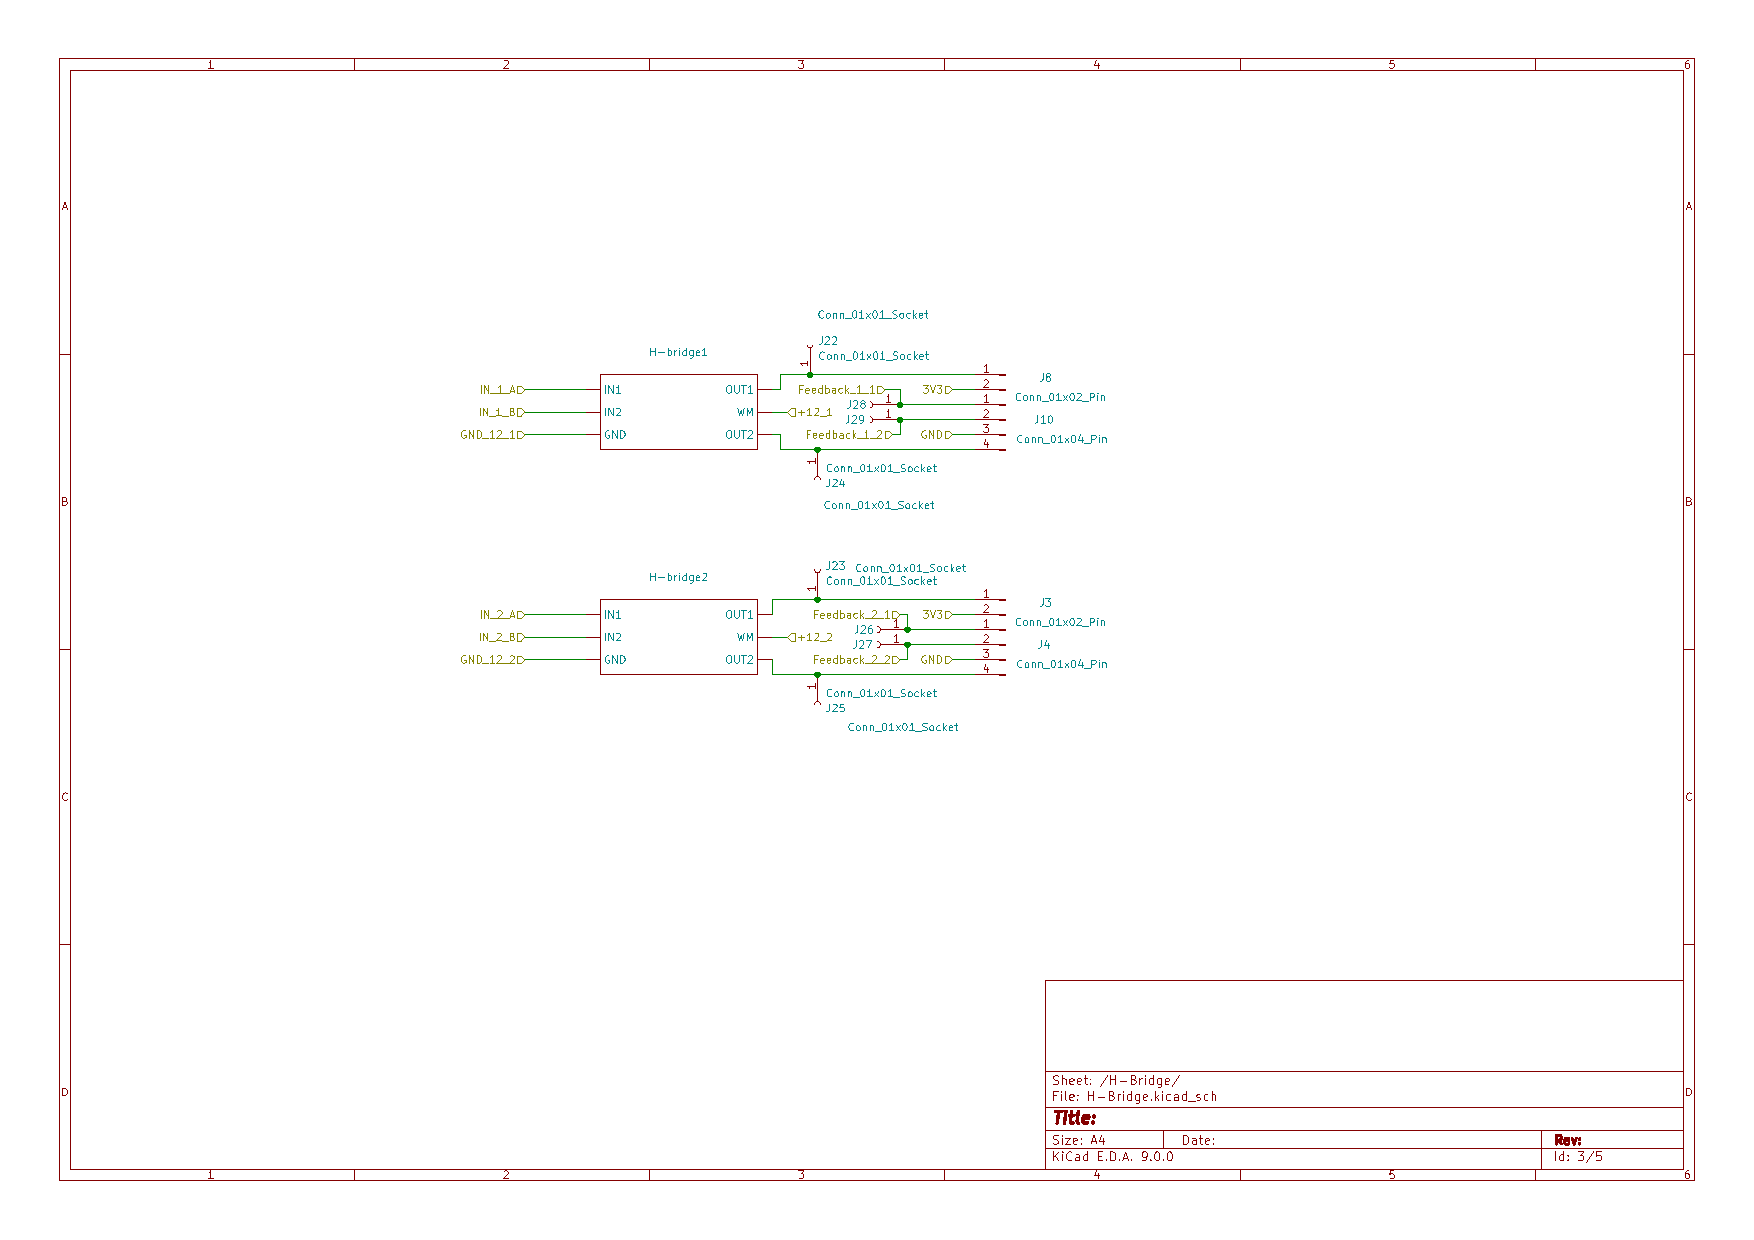
\includepdf[angle = -90]{obrazky/old_schematic-H-Bridge.pdf}
\subsection{ESP}
Tento list obsahuje zapojení mikrokontroleru ESP32, všech sériových komunikací, SD karty přípravu pro akcelerometr. Během zapojování však na mikrokontroleru došly piny a bylo nutné najít vhodnou alternativu. Tomuto problému se věnuje úvod a první podkapitola následující kapitoly.


\newpage
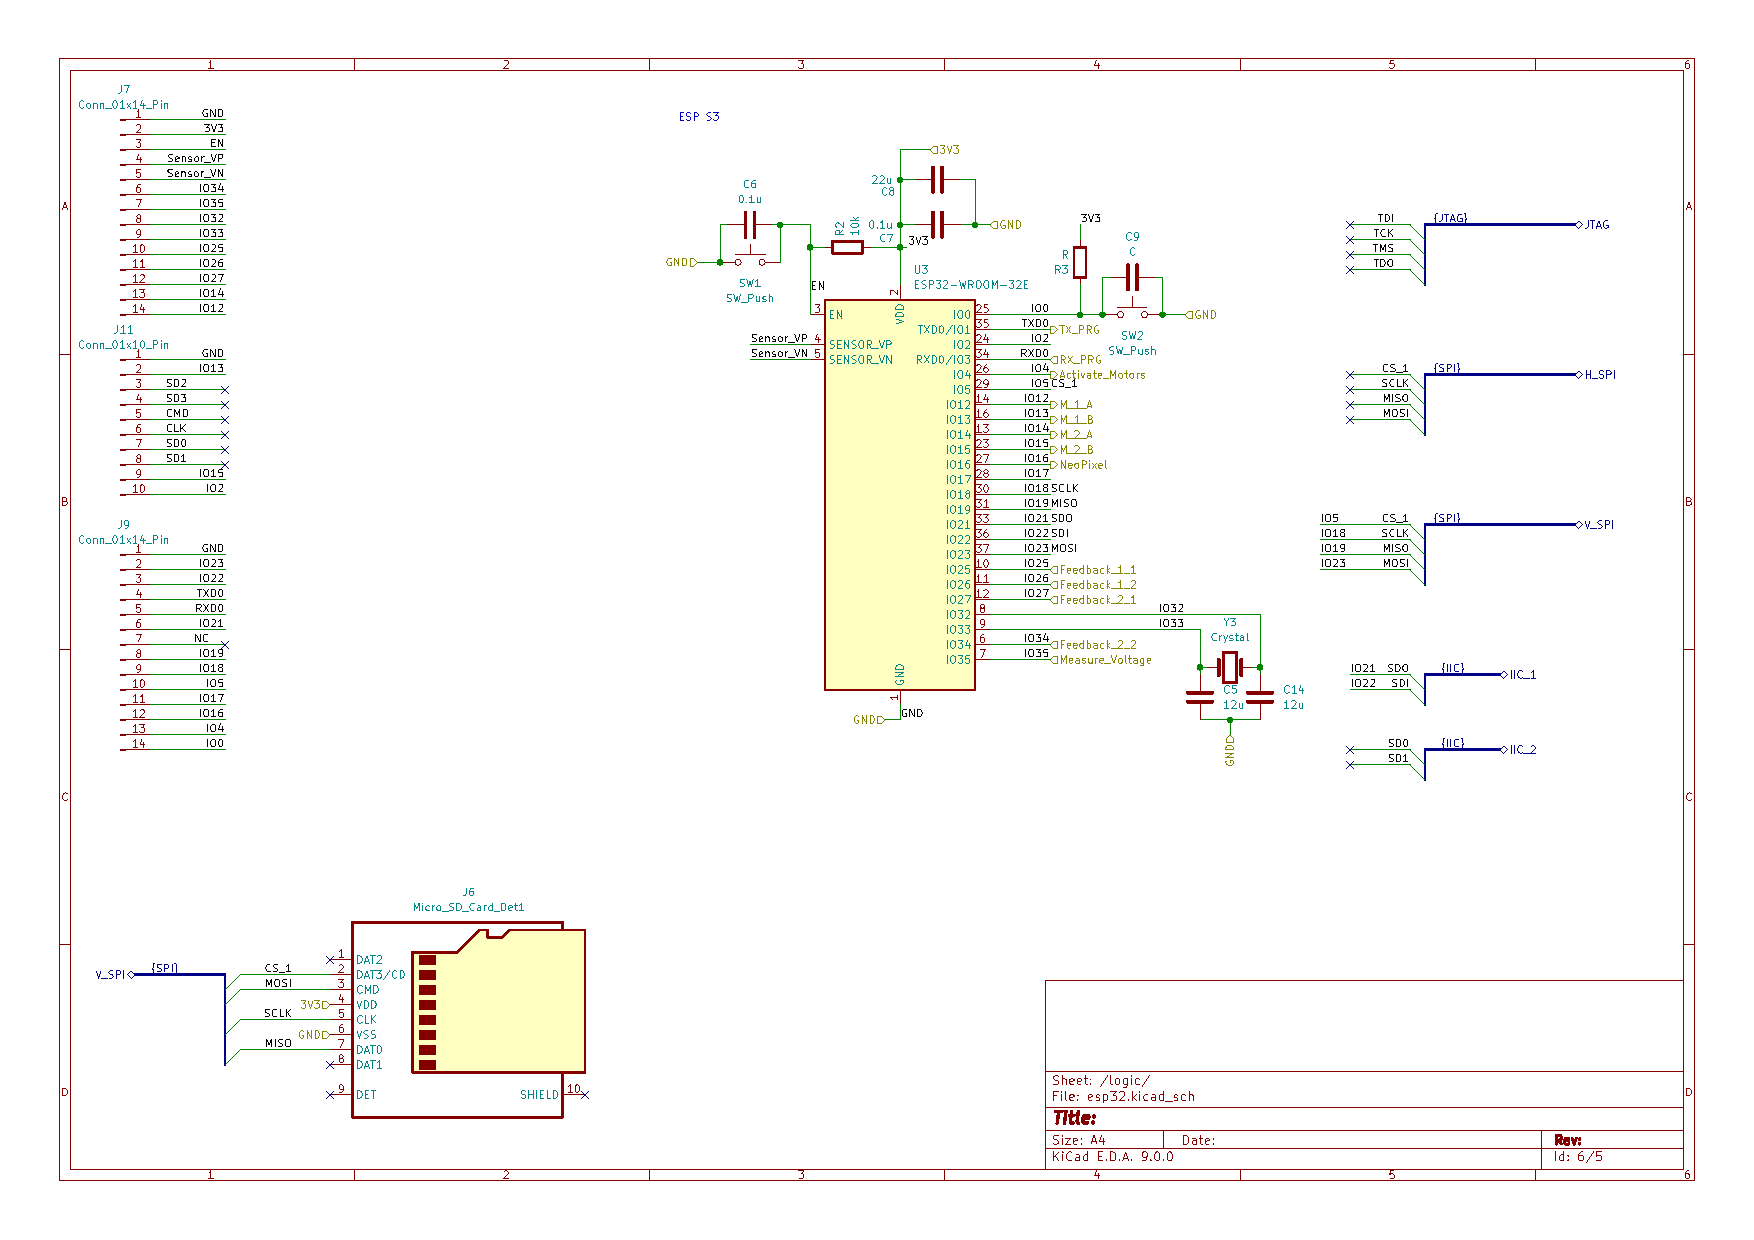
\includepdf[angle = -90]{obrazky/old_schematic-logic.pdf}
\subsection{PSU}
Poslední list schématu obsahuje schémata potřebná pro napájení robota. Nachází se zde dva step up moduly s připojenými filtračními kondenzátory a špičkovým napětím pomocí zenerovy diody. Při vysokofrekvenčním spínání motoru pomocí H můtku by mohly být generovány poměrně vysoké napěťové špičky. Poro jistotu zde byly umístěny tyto ochrany.
Step up moduly jsou spínány pomocí dvou MOSFET tranzistorů. Tyto tranzistory mají při otevření téměř nulový odpor. Jsou tedy vhodné pro spínání obvodů se zvýšenou spotřebou. Přoč jsou zde potřeba? Při chybě programu by mohlo dojít k nekontrolovanému otáčení motorů. Záréveň také není vhodné, aby se motory náhodou spustily při programování, či nabíjení robota. Byla zde tedy implementována ochrana.
Další částí schématu je integrovaný obvod pro nabíjení článků 18650. Ty jsou připojeny přes modul \ac{bms}. Tento modul zajišťuje rovnoměrné zatížení obou článků. Zároveň se stará o balancování článků při nabíjení. Tento modul obsahuje také ochranu proti přetížení, přepětí, či přílišnému vybití.
Poslední částí jsou lineární regulátory pro logiku. Ty z 6-8.4V nacházejících se na výstupu akumulátoru vytváří 3.3 a 5V pomocí principu lineární regulace. Přebytečnou energii jednoduše přemění na teplo.
\newpage
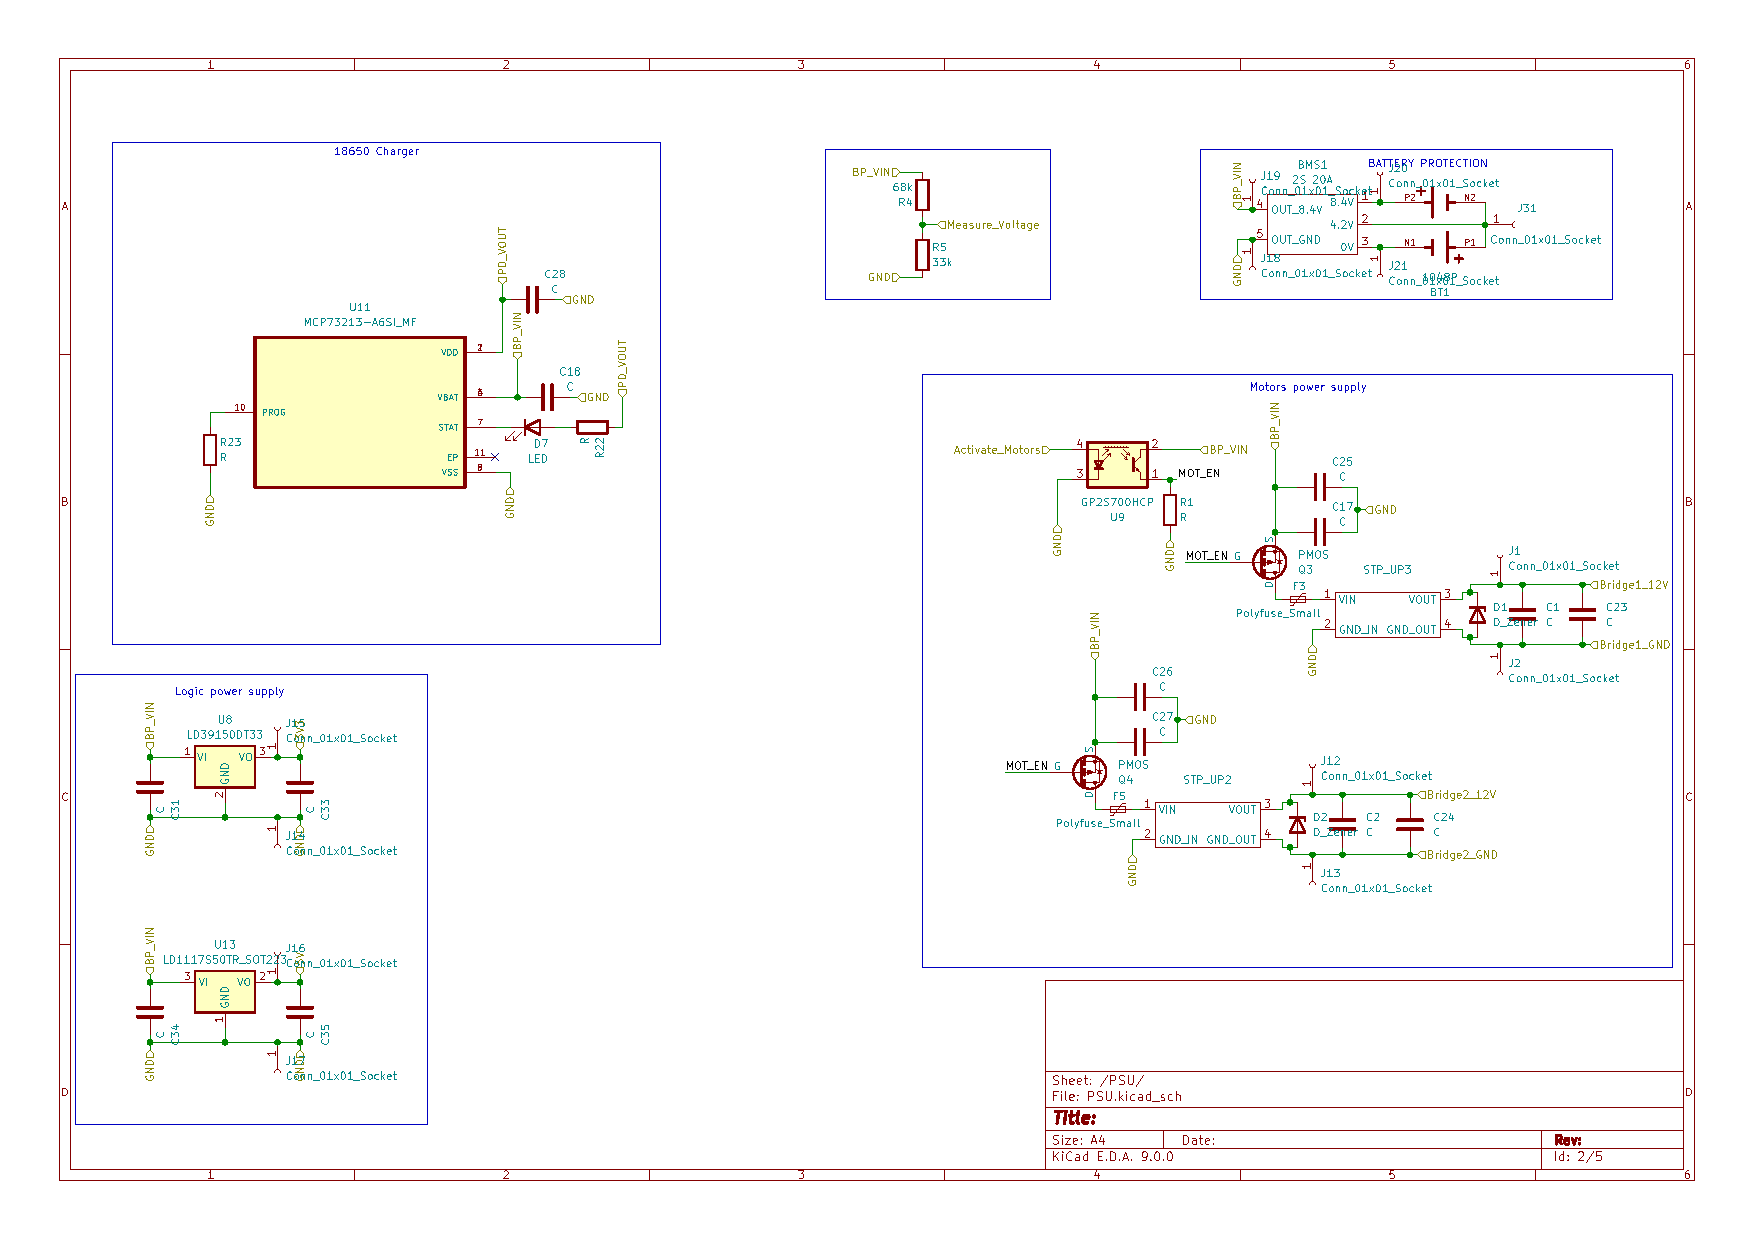
\includepdf[angle = -90]{obrazky/old_schematic-PSU.pdf}